% File: intro.tex
% Date: Sun May 05 16:58:35 2013 +0800
% Author: Yuxin Wu <ppwwyyxxc@gmail.com>
\section{Usage}
The program is written in C++11, and is also available at \url{https://github.com/ppwwyyxx/panorama}.

\subsection{Compilation}
Dependencies:

\begin{enumerate}
    \item gcc >= 4.7
    \item GNU make
    \item Magick++
    \item boost MTL (Matrix Template Library) installed in /usr/include/boost/numeric/.
      It can be downloaded from \url{http://www.simunova.com/node/145}. A copy is attached in the submitted package.
\end{enumerate}

Compilation:
\begin{lstlisting}
$ make
\end{lstlisting}

\subsection{Run}
Various parameters are saved in \verb|src/config.cfg|.
Without special needs, we only have to modify \verb|PANO, TRANS, CROP|.

The program does some extra work to beautify the output
if knowing the input pictures were taken by a camera
moving in pure translation or pure rotation.

\verb|PANO = 1| tells that the camera moved in pure rotation. A panorama is expected to be the output;

\verb|TRANS = 1| tells that the camera moved in pure translation. Result will be better than the one with \verb|TRANS| unset;

\verb|CROP| decides whether to crop the final image to a rectangular;

Use \verb|./main <file1> <file2> <file3> ...| in the command line to run the program.
Output file is \verb|out.png|.

Usually, input images should not exeeds $20(files)\times 1500(pixels) \times 1000(pixels)$, since your computer may not have enough memory.

The input file names given in the command line need to be well ordered, to make sure the adjacent images can be stitched together.

\subsection{Examples}
\begin{enumerate}
\item TRANS = 1
  \begin{lstlisting}
$ ./main ../data/flower/small*
  \end{lstlisting}
\begin{figure}[H]
  \centering
  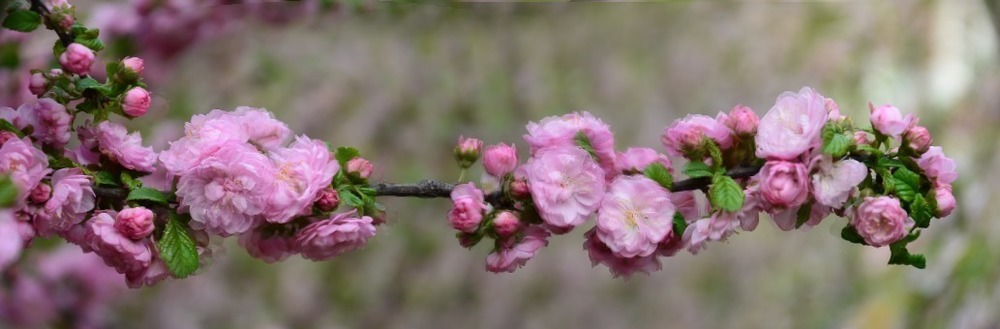
\includegraphics[scale=0.27]{res/small.png}
\end{figure}


  \item PANO = 1
    \begin{lstlisting}
$ ./main ../data/ground/small*
    \end{lstlisting}
    The result is shown in \figref{cropped}.
\end{enumerate}
